
\documentclass{article}
\usepackage{graphicx} % Required for inserting images
\usepackage{fancyhdr} % Required for header and footer configuration
\usepackage[a4paper, margin=2.5cm, left=1.5cm, right=1.5cm, bottom=4cm]{geometry} % Required for setting page margins
\usepackage[T1]{fontenc}
\usepackage[default,oldstyle,scale=1]{opensans} % Utilizzo del font Open Sans
\usepackage{lipsum}
\usepackage{makeidx}
\usepackage{booktabs}
\usepackage{tabularray}
\usepackage[colorlinks=true, linkcolor=black, urlcolor=blue, citecolor=blue]{hyperref}
\usepackage{tabularx}
\usepackage{makecell}
\usepackage{enumitem} % Pacchetto per la personalizzazione degli elenchi
\usepackage{booktabs}
\usepackage{subcaption}

% Configure header and footer for the first page
\fancypagestyle{firstpage}{
    \fancyhf{} % Clear header and footer
    \renewcommand{\headrulewidth}{0pt} % Remove header rule line
    \lhead{} % Header on the left
    \chead{} % Header in the center
    \rhead{} % Header on the right
    \lfoot{} % Footer on the left
    \cfoot{\vspace{5pt}\\\hrulefill\\\vspace{10pt}\textbf{BeeLive}\\Gruppo 21} % Footer in the center
    \rfoot{\vspace{32.5pt}\\\thepage} % Footer on the right
}

% Configure header and footer for non-plain pages (second page onwards)
\fancypagestyle{nonplain}{
    \fancyhf{} % Clear header and footer
    \lhead{} % Header on the left
    \chead{} % Header in the center
    \rhead{
\includegraphics[width=2cm]{Images/BeeLive-Logo.png}\\\vspace{2pt}} % Header on the right
    \lfoot{} % Footer on the left
    \cfoot{\vspace{5pt}\\\hrulefill\\\vspace{10pt}\textbf{BeeLive}\\Gruppo 21} % Footer in the center
    \rfoot{\vspace{32.5pt}\\\thepage} % Footer on the right
}

% Adjust vertical space between header and text                                    
\setlength{\headsep}{65pt} 
% Adjust vertical space between text and footer
\setlength{\footskip}{0pt} 

\title{
\includegraphics[width=0.75\textwidth]{Images/BeeLive-Logo.png}\\\vspace{100pt}
\LARGE{\textbf{BeeLive\\Deliverable 2}}}
\author{Gruppo 21:\\
Cipriani Pietro, 226959\\
Orlando Dennis, 227688\\
Ziviani Elia, 228172}
\date{22 Aprile 2024}

\makeindex % Indica che vogliamo creare un indice

\begin{document}

\maketitle
\thispagestyle{firstpage} % Apply firstpage style to the first page
\clearpage

\pagestyle{nonplain} % Apply non-plain style to subsequent pages

\renewcommand{\contentsname}{Indice}
\tableofcontents

\clearpage

\section{Component Diagram}
\index{Component Diagram}

Questo capitolo è incentrato sull'analisi dei componenti del sistema che saranno realizzati.\\
Lo scopo è quello di descrivere ogni singolo componente in termini di funzionalità e interfacce.\\

I componenti sono individuati seguendo quando espresso nel documento Deliverable 1 per quanto riguarda i casi d'uso e sono definiti come entità autonome nel sistema.\\
Questi componenti sono provvisti di interfacce che permettono la comunicazione tra di essi.\\
Le interfacce sono definite come:
\begin{itemize}
    \item \textbf{Interfacce di OUTPUT}: Tutte quelle interfacce che offrono servizi al sistema.
    \item \textbf{Interfacce di INPUT}: Tutte quelle interfacce che ricevono servizi dal sistema.
\end{itemize} 

\subsection{Gestione }
\index{Gestione}

\begin{table}[htbp]
    \centering
    \begin{tabularx}{\textwidth}{| l | l | p{0.8075\textwidth} |}
        \Xhline{2pt}
        INPUT & Nome & Descrizione \\
        \Xhline{2pt}
        Ciao & a & tutti \\
        \Xhline{2pt}
        Output & Nome & Descrizione \\
        \Xhline{2pt}
        Ciao & a & tutti \\
        \hline
    \end{tabularx}
    \caption{Registrazione ed autenticazione dell' utente anonimo}
\end{table}

%---------------------------------
\begin{table}[htbp]
    \centering
    \begin{tabularx}{\textwidth}{| l | l | p{0.8075\textwidth} |}
        \Xhline{2pt}
        INPUT & Nome & Descrizione \\
        \Xhline{2pt}
        Ciao & a & tutti \\
        \Xhline{2pt}
        Output & Nome & Descrizione \\
        \Xhline{2pt}
        Ciao & a & tutti \\
        \hline
    \end{tabularx}
    \caption{Registrazione ed autenticazione dell' utente anonimo}
\end{table}

\begin{figure}[htbp]
    \centering
    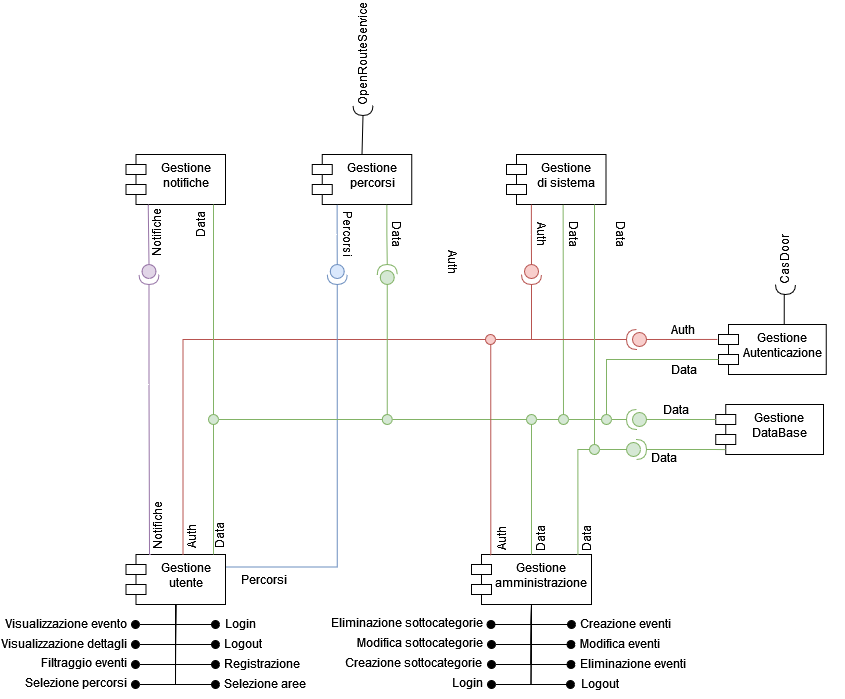
\includegraphics[width=1\textwidth]{Images/ComponentDiagram.png}
    \caption{Diagramma dei componenti}
    \label{fig:component-diagram}
\end{figure}

\end{document}